\section{Future Work}

\subsection{Expand Library of Primitives}
In this paper we have made many simplifications to the problem space just to make the placer easier to implement.
For example, our placer in its current state does not take advantage of \texttt{SLICEL}/\texttt{SLICEM} homogeneity and simply maps all SLICE \texttt{SiteInst}s onto \texttt{SLICEL}s. 
Recall that the SLICE Sites in Xilinx FPGAs typically come in a 75-25\% split between \texttt{SLICEL}s and \texttt{SLICEM}s. 
This means that we have rendered about 25\% of the CLB fabric unusable which will inevitably hurt wirelength minimization during placement since the \texttt{SiteInst}s must be spread over a larger area. 

\subsection{Robustness}
In its current state, the prepacker and packer struggle with data busses larger than 24-bits, especially with DSP functions like addition and multiplication. 

\subsection{Improvements to Packing}
There is also no rule saying we must pack \texttt{Cells} into \texttt{SiteInst}s before placement or that we follow a strict prepacking-packing-placement flow. 

{
    \centering
    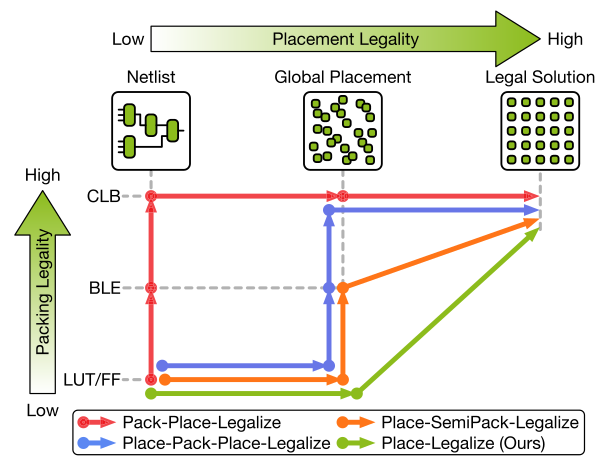
\includegraphics[width=\columnwidth]{figures/future_work/legalization.png}
    \captionof{figure}{Representative FPGA placement and packing flows. Figure taken from Wuxi et al. (2019), page 1 \cite{ExplicitPacking}}
}
\vspace{0.25cm}


The latest editions of Vivado performs BEL-centric placement without necessarily locking \texttt{Cell}s into \texttt{Site}s, allowing a higher granularity of movement of \texttt{Cell}s during placement. 

\subsection{Improvements to SA}

\subsection{Force-Directed and Analytical Placement}

In more sophisticated placers, the proposed movement can also be selected by finding the centroid between \texttt{SiteInst}s that share a net with the current object, or even a hybrid of random and centroid selection. 
We will implement variations on the vanilla SA algorithm that use centroid selection. 
Moves that actively attempt to predict a better placement are often referred to as "directed" moves in literature. 
Placers that take inspiration from physical interactions like gravity or electrostatics are often referred to as "force directed" placers and are akin to physics simulators. 

Directed moves as opposed to undirected moves give rise to the concept of legalization. 
When using undirected moves as in SA, we can simply keep track of a \texttt{List} or \texttt{HashMap} of occupied \texttt{Site}s and available \texttt{Site}s and select from that data structure via random selection. 
However, for directed moves like centroid selection, the centroid between \texttt{Site}s may not necessarily fall directly on another discrete \texttt{Site} on the \texttt{device}. 
Even when it does, the centroid \texttt{Site} may be incompatible with the \texttt{SiteInst} or may fail to meet some other placement constraint. 
In such cases, we must do a neighborhood search around the centroid up to a certain radius to find a \texttt{Site} that satisfies all the constraints of the \texttt{SiteInst} at hand. 
We will take some inspiration from ray-marching in graphics and do a diamond-shaped spiral search around the centroid where we check the legality of each \texttt{Site} as we step through the spiral and select the first \texttt{Site} that meets all of the placement constraints. 

In force directed placers, there is a concept of global placement followed by detailed placement.
Global placement places object instances freely on an analog plane and is driven purely by directed movement and analytical solution.
In global placement stage, only non-hardware related objectives are considered. 
Object instance placements do not have to adhere to any hardware constraints and can even overlap with one another.
Afterwards, detailed placement "legalizes" the global placement by discretizing the analog positions of the instances onto the discrete grid of resources of the \texttt{device}.
Overlapping instances are iteratively spread out until every \texttt{SiteInst}-\texttt{Cell} is assigned its own unique \texttt{Site}-\texttt{BEL}.
The spreading process somewhat resembles primitive fluid dynamics simulators or thermal diffusion simulators, where packets of energy are spread through a medium until each voxel or pixel of the medium falls below a maximum threshold of energy. 
There also exists other strategies to mix packing, placement, and legalization in different orders, such as those studied in \cite{ExplicitPacking}. 
In this context, our placer follows a very straightforward pack-legalize-place strategy with SA. 




